\documentclass[]{book}
\usepackage[T1]{fontenc}
\usepackage{lmodern}
\usepackage{amssymb,amsmath}
\usepackage{ifxetex,ifluatex}
\usepackage{fixltx2e} % provides \textsubscript
\usepackage{booktabs}

\providecommand{\tightlist}{%
  \setlength{\itemsep}{0pt}\setlength{\parskip}{0pt}}

% use upquote if available, for straight quotes in verbatim environments
\IfFileExists{upquote.sty}{\usepackage{upquote}}{}
\ifnum 0\ifxetex 1\fi\ifluatex 1\fi=0 % if pdftex
  \usepackage[utf8]{inputenc}
\else % if luatex or xelatex
  \ifxetex
    \usepackage{mathspec}
    \usepackage{xltxtra,xunicode}
  \else
    \usepackage{fontspec}
  \fi
  \defaultfontfeatures{Mapping=tex-text,Scale=MatchLowercase}
  \newcommand{\euro}{€}
\fi
% use microtype if available
\IfFileExists{microtype.sty}{\usepackage{microtype}}{}
\usepackage{color}
\usepackage{fancyvrb}
\newcommand{\VerbBar}{|}
\newcommand{\VERB}{\Verb[commandchars=\\\{\}]}
\DefineVerbatimEnvironment{Highlighting}{Verbatim}{commandchars=\\\{\}}
% Add ',fontsize=\small' for more characters per line
\newenvironment{Shaded}{}{}
\newcommand{\KeywordTok}[1]{\textcolor[rgb]{0.00,0.44,0.13}{\textbf{{#1}}}}
\newcommand{\DataTypeTok}[1]{\textcolor[rgb]{0.56,0.13,0.00}{{#1}}}
\newcommand{\DecValTok}[1]{\textcolor[rgb]{0.25,0.63,0.44}{{#1}}}
\newcommand{\BaseNTok}[1]{\textcolor[rgb]{0.25,0.63,0.44}{{#1}}}
\newcommand{\FloatTok}[1]{\textcolor[rgb]{0.25,0.63,0.44}{{#1}}}
\newcommand{\ConstantTok}[1]{\textcolor[rgb]{0.53,0.00,0.00}{{#1}}}
\newcommand{\CharTok}[1]{\textcolor[rgb]{0.25,0.44,0.63}{{#1}}}
\newcommand{\SpecialCharTok}[1]{\textcolor[rgb]{0.25,0.44,0.63}{{#1}}}
\newcommand{\StringTok}[1]{\textcolor[rgb]{0.25,0.44,0.63}{{#1}}}
\newcommand{\VerbatimStringTok}[1]{\textcolor[rgb]{0.25,0.44,0.63}{{#1}}}
\newcommand{\SpecialStringTok}[1]{\textcolor[rgb]{0.73,0.40,0.53}{{#1}}}
\newcommand{\ImportTok}[1]{{#1}}
\newcommand{\CommentTok}[1]{\textcolor[rgb]{0.38,0.63,0.69}{\textit{{#1}}}}
\newcommand{\DocumentationTok}[1]{\textcolor[rgb]{0.73,0.13,0.13}{\textit{{#1}}}}
\newcommand{\AnnotationTok}[1]{\textcolor[rgb]{0.38,0.63,0.69}{\textbf{\textit{{#1}}}}}
\newcommand{\CommentVarTok}[1]{\textcolor[rgb]{0.38,0.63,0.69}{\textbf{\textit{{#1}}}}}
\newcommand{\OtherTok}[1]{\textcolor[rgb]{0.00,0.44,0.13}{{#1}}}
\newcommand{\FunctionTok}[1]{\textcolor[rgb]{0.02,0.16,0.49}{{#1}}}
\newcommand{\VariableTok}[1]{\textcolor[rgb]{0.10,0.09,0.49}{{#1}}}
\newcommand{\ControlFlowTok}[1]{\textcolor[rgb]{0.00,0.44,0.13}{\textbf{{#1}}}}
\newcommand{\OperatorTok}[1]{\textcolor[rgb]{0.40,0.40,0.40}{{#1}}}
\newcommand{\BuiltInTok}[1]{{#1}}
\newcommand{\ExtensionTok}[1]{{#1}}
\newcommand{\PreprocessorTok}[1]{\textcolor[rgb]{0.74,0.48,0.00}{{#1}}}
\newcommand{\AttributeTok}[1]{\textcolor[rgb]{0.49,0.56,0.16}{{#1}}}
\newcommand{\RegionMarkerTok}[1]{{#1}}
\newcommand{\InformationTok}[1]{\textcolor[rgb]{0.38,0.63,0.69}{\textbf{\textit{{#1}}}}}
\newcommand{\WarningTok}[1]{\textcolor[rgb]{0.38,0.63,0.69}{\textbf{\textit{{#1}}}}}
\newcommand{\AlertTok}[1]{\textcolor[rgb]{1.00,0.00,0.00}{\textbf{{#1}}}}
\newcommand{\ErrorTok}[1]{\textcolor[rgb]{1.00,0.00,0.00}{\textbf{{#1}}}}
\newcommand{\NormalTok}[1]{{#1}}
\usepackage{graphicx}
% Redefine \includegraphics so that, unless explicit options are
% given, the image width will not exceed the width of the page.
% Images get their normal width if they fit onto the page, but
% are scaled down if they would overflow the margins.
\makeatletter
\def\ScaleIfNeeded{%
  \ifdim\Gin@nat@width>\linewidth
    \linewidth
  \else
    \Gin@nat@width
  \fi
}
\makeatother
\let\Oldincludegraphics\includegraphics
{%
 \catcode`\@=11\relax%
 \gdef\includegraphics{\@ifnextchar[{\Oldincludegraphics}{\Oldincludegraphics[width=\ScaleIfNeeded]}}%
}%
\ifxetex
  \usepackage[setpagesize=false, % page size defined by xetex
              unicode=false, % unicode breaks when used with xetex
              xetex]{hyperref}
\else
  \usepackage[unicode=true]{hyperref}
\fi
\hypersetup{breaklinks=true,
            bookmarks=true,
            pdfauthor={Karl Benedict},
            pdftitle={Geography 485L/585L Weekly Breakdown},
            colorlinks=true,
            citecolor=blue,
            urlcolor=blue,
            linkcolor=magenta,
            pdfborder={0 0 0}}
\urlstyle{same}  % don't use monospace font for urls
\setlength{\parindent}{0pt}
\setlength{\parskip}{6pt plus 2pt minus 1pt}
\setlength{\emergencystretch}{3em}  % prevent overfull lines

\oddsidemargin = 0pt
\evensidemargin = 0pt
\topmargin = -36pt
\textwidth = 468pt
\textheight = 648pt

\setcounter{secnumdepth}{0}

\title{Geography 485L/585L Weekly Breakdown}
\author{Karl Benedict}
\date{Spring 2016}

\begin{document}
\maketitle

{
\hypersetup{linkcolor=black}
\setcounter{tocdepth}{2}
\tableofcontents
}
\chapter{Goals and Objectives}\label{goals}

Internet mapping technologies are an important component of geospatial
data capture, sharing, visualization, and delivery. This course provides
a survey of current and emerging internet and geospatial
interoperability standards, technologies, and capabilities. The emphasis
of the work in this class will be hands-on experience in four critical
aspects of Internet-enabled mapping:

\begin{itemize}
\item
  The basic concepts behind web development and web mapping technologies
  that enable the delivery of maps and mapped data through web browsers
\item
  The Open Standards that facilitate the exchange of map images and
  geospatial data over the internet
\item
  The use of published standards-based services in desktop mapping
  applications that implement those standards
\item
  The deployment of standards-based geospatial map and data services
  that other systems and users may make use of
\end{itemize}

The specific class objectives that relate to these activities and
departmental curriculum objectives for undergraduate and graduate
students in the Geography Department include the following:

\begin{itemize}
\item
  Students will understand the concepts geospatial data and service
  interoperability
\item
  Students will be able to define the specific requirements of a
  particular analysis or project and identify the interoperability
  standards that are capable of meeting those requirements
\item
  Students will be knowledgeable in the core technologies that they may
  use to produce their own internet-enabled mapping capabilities
\item
  Students will understand the strengths and limitations of current
  internet mapping technologies for generating cartographically
  effective map products.
\end{itemize}

The weekly goals, objectives and assignments are outlined below

\chapter{Week 1 - Introductions, Course Outline \& Web
Concepts}\label{week01}

This week we will review the content and structure for the course and
spend some time getting to know each other. Following this we will spend
some time setting up some of the tools that you will be using for the
course in developing your portfolio of materials.

\section{Class Prep}\label{week01-prep}

\begin{itemize}
\item
  \href{http://en.wikipedia.org/wiki/History_of_the_World_Wide_Web}{Wikipedia
  article - History of the World Wide web}
\item
  \href{http://www.lynda.com/SharedPlaylist/2b710369c9ec4d8c964467225c6610ad?org=unm.edu}{Lynda.com
  tutorials}

  \begin{itemize}
  \tightlist
  \item
    \emph{Web Design Fundamentals}

    \begin{itemize}
    \item
      Introduction
    \item
      \begin{enumerate}
      \def\labelenumi{\arabic{enumi}.}
      \tightlist
      \item
        Exploring Web Design
      \end{enumerate}
    \end{itemize}
  \item
    \emph{Version Control for Everyone}

    \begin{itemize}
    \item
      Introduction
    \item
      \begin{enumerate}
      \def\labelenumi{\arabic{enumi}.}
      \tightlist
      \item
        Introducing Version Control
      \end{enumerate}
    \item
      \begin{enumerate}
      \def\labelenumi{\arabic{enumi}.}
      \setcounter{enumi}{1}
      \tightlist
      \item
        Version Control Basics
      \end{enumerate}
    \item
      \begin{enumerate}
      \def\labelenumi{\arabic{enumi}.}
      \setcounter{enumi}{2}
      \tightlist
      \item
        Setting Up Your First Project
      \end{enumerate}
    \end{itemize}
  \end{itemize}
\end{itemize}

\section{Reference Materials}\label{week01-reference}

\href{https://github.com/UNM-GEOG-485-585/class-materials/raw/master/syllabus.pdf}{Class
Syllabus}

\section{Weekly Milestone - Creating Your GitHub Repository and First
Web Page}\label{week01-milestone}

Developing content to go onto the web has evolved from a solitary effort
to one where teams work together in developing components of larger web
sites. These teams need to have a variety of tools to enable their work.
Some of the most important tools enable code sharing with the team, and
in projects based on the \href{http://opensource.org/osd-annotated}{Open
Source} software model the rest of the world. The
\href{https://github.com/}{GitHub} web platform uses the
\href{http://git-scm.com/}{Git} distributed
\href{http://en.wikipedia.org/wiki/Revision_control}{version control}
system to enable sharing of code and hosting static web pages based on
that shared code.

You will be using a private \href{http://github.com}{GitHub} repository
to build your class portfolio during the course. If you would like to
make your portfolio available publicly you can also use GitHub as the
platform for providing that public access. Regardless of your decision
about providing public access to your portfolio, you will learn how
version control operates, and how to provide comments and keep notes on
your work and comment on the work of others (this will be part of our
peer review process).

While the work we do this and next week will be directly through the
editor integrated into the GitHub system, you will eventually need to
install a desktop application (such as the
\href{https://www.sourcetreeapp.com/}{SourceTree} application
recommended for the class) that allows you to develop your web pages on
your local computer and then update the files on the GitHub system when
you want to share a new version. Also, you can't add things like images
to your web pages until you are adding them to a local repository on
your computer and then sending them GitHub.

For this milestone we will walk through the process of creating your
repository in GitHub, creating your first web page, previewing that page
on your local computer, changing the page, and updating the page on
LoboGit. For this milestone we will do this as a manual process which we
will streamline in the coming weeks.

\emph{Step 1} - Create Your GitHub Account and Portfolio Repository

For your work in this class you will build your portfolio within an
organization (\url{https://github.com/UNM-GEOG-485-585}) within GitHub
that has been created for the class. The first step in the process of
creating your portfolio is to create a new \emph{repository} in GitHub
within which you will put your portfolio materials for sharing within
the class. Please follow the following steps to create your repository:

\begin{enumerate}
\def\labelenumi{\arabic{enumi}.}
\tightlist
\item
  Go to the \href{https://github.com/}{GitHub homepage} and follow the
  onscreen instructions for creating a new account. If you already have
  an account you can skip this step.
\item
  Come to the front of the class and tell me your GitHub username so
  that I can add you to the organization and create your repository for
  you within the organization.
\end{enumerate}

\emph{Step 2} - Create Your First Web Page

To create your first web page within your portfolio repository you need
to first enter your repository, add a new file, modify its contents, and
commit your modifications back to the repository to save your changes.

\begin{enumerate}
\def\labelenumi{\arabic{enumi}.}
\tightlist
\item
  Go to the class organization page
  ((\url{https://github.com/UNM-GEOG-485-585} - logging in if necessary)
  and click on your repository name in the list.
\item
  On the page that comes up listing the files in your repository, click
  the ``New File'' button above the list of files.
\end{enumerate}

\begin{figure}[htbp]
\centering
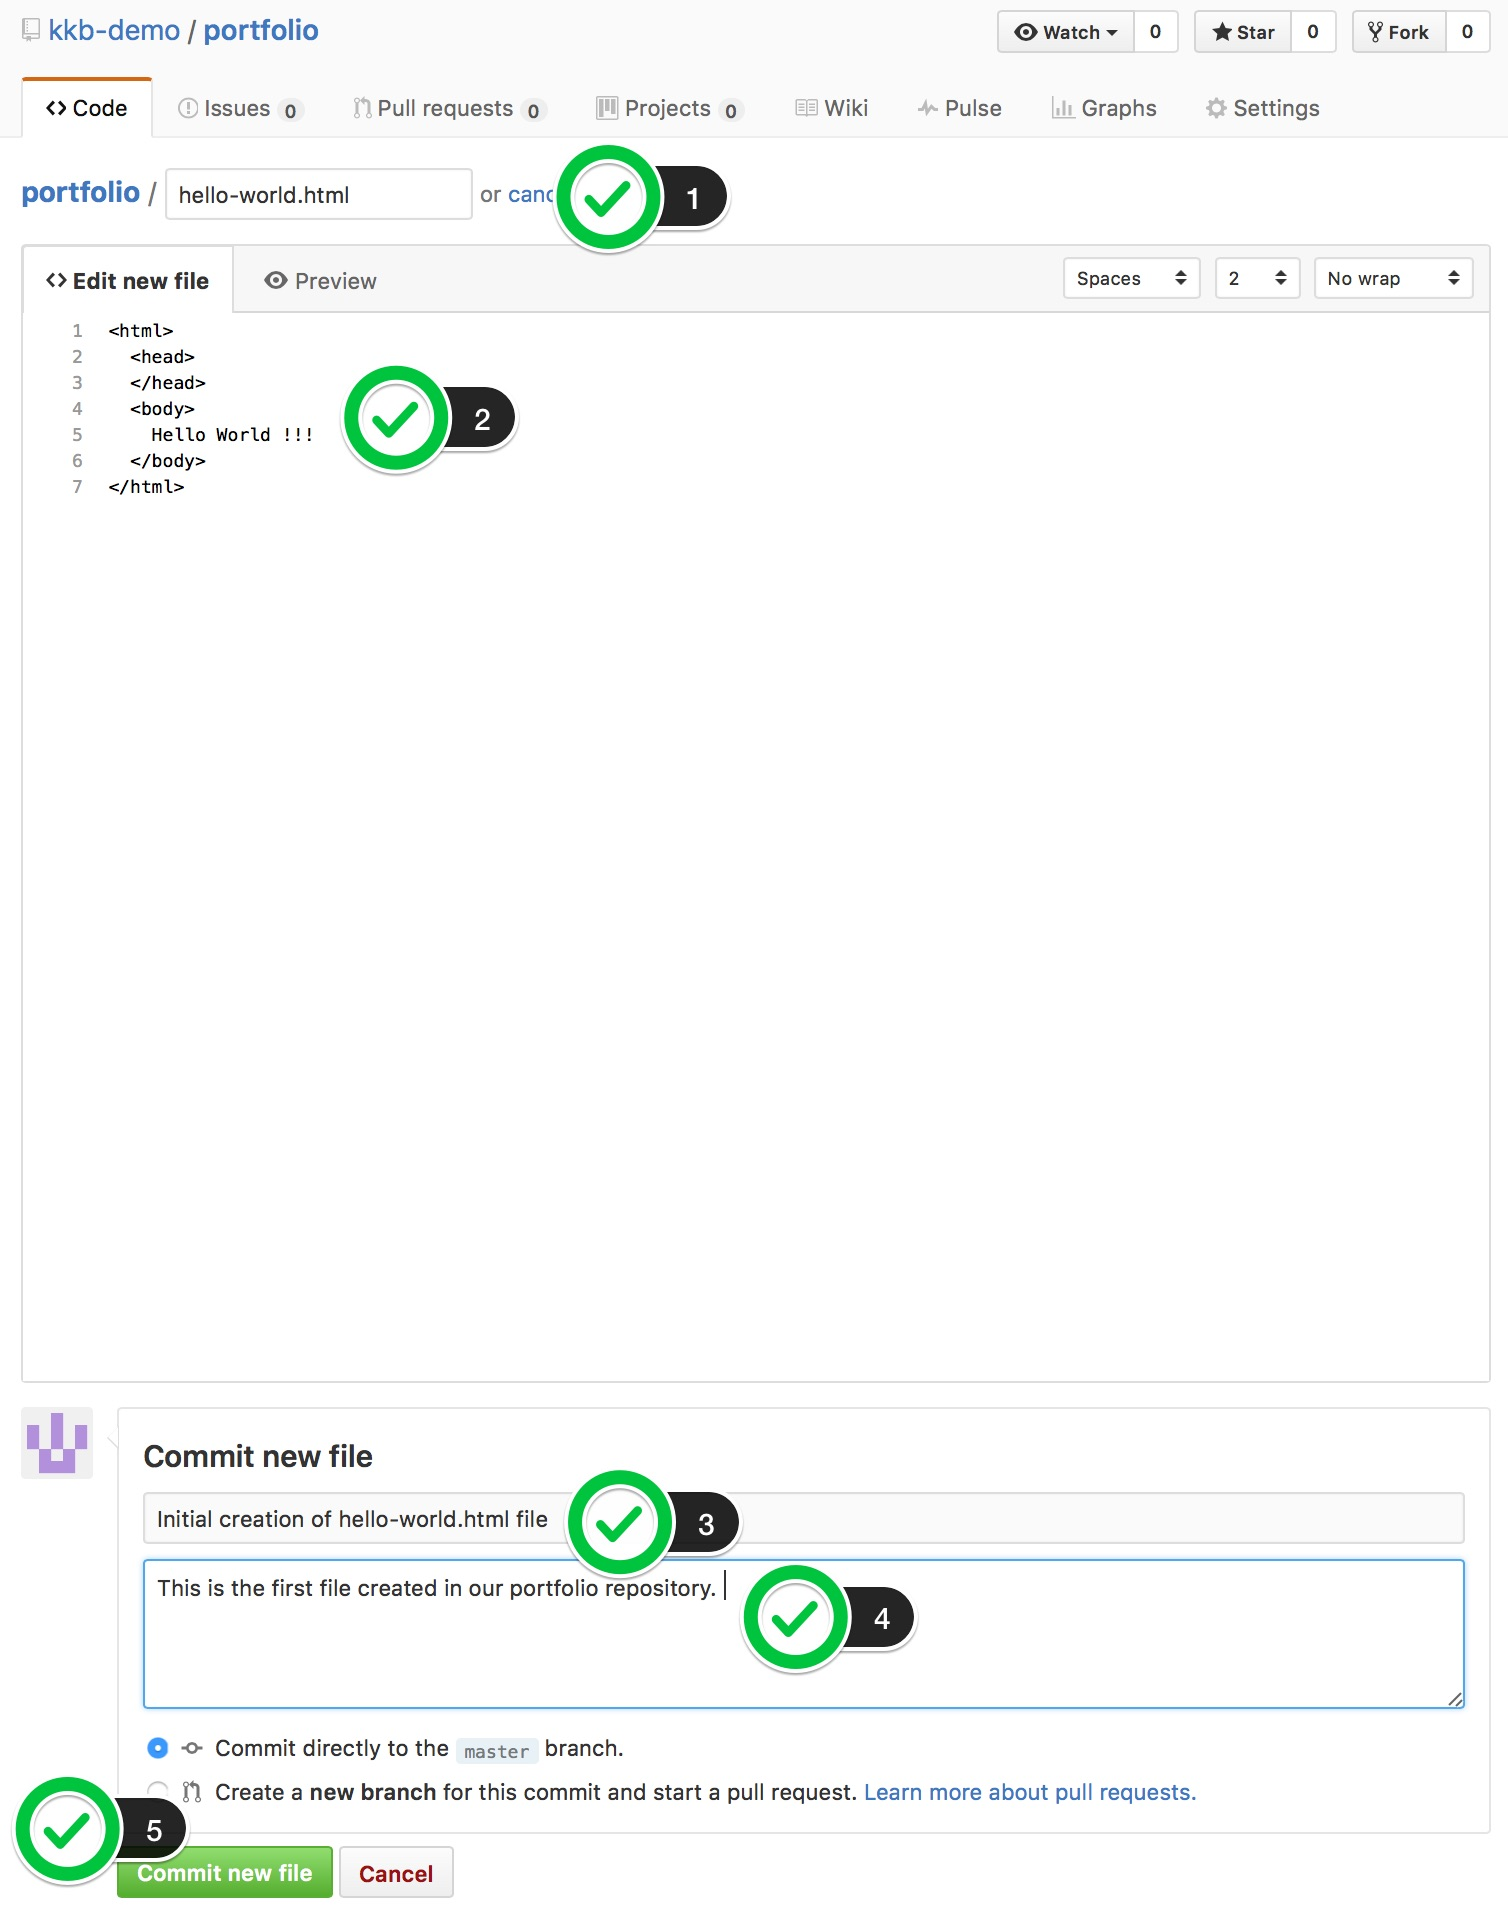
\includegraphics[width=0.70000\textwidth]{images/github_editor.png}
\caption{GitHub file creation/editor page}
\end{figure}

\begin{enumerate}
\def\labelenumi{\arabic{enumi}.}
\setcounter{enumi}{2}
\tightlist
\item
  Enter the name of the file that you are creating as
  ``hello-world.html''
\item
  Enter the following text into the text entry area under the filename
  field.
\end{enumerate}

\begin{Shaded}
\begin{Highlighting}[numbers=left,,]
\KeywordTok{<html>}
    \KeywordTok{<head>}
    \KeywordTok{</head>}     
    \KeywordTok{<body>}
        \NormalTok{Hello World !!!}
    \KeywordTok{</body>} 
\KeywordTok{</html>}
\end{Highlighting}
\end{Shaded}

\begin{enumerate}
\def\labelenumi{\arabic{enumi}.}
\setcounter{enumi}{4}
\tightlist
\item
  Add a brief comment (such as ``Created hello-world.html from provided
  text'') in the first field under the ``Commit new file'' title. You
  can optionally add a more detailed description in the next field if
  you like.
\item
  Keep the default option to ``Commit directly to the master branch''
\item
  Click the ``Commit New File'' button to commit your change and save
  the file
\end{enumerate}

\emph{Step 3} - Preview Your Web Page in a Browser

While we will later discuss strategies for hosting your web content on a
system (GitHub for example) that supports direct access by web clients,
to preview the web page you just created you need to download the
repository to your local computer where you can open the locally stored
file in a browser.

\begin{enumerate}
\def\labelenumi{\arabic{enumi}.}
\tightlist
\item
  Go to the class organization page
  ((\url{https://github.com/UNM-GEOG-485-585} - logging in if necessary)
  and click on your repository name in the list.
\item
  On the page that comes up listing the files in your repository, click
  the ``Download Zip'' button above the list of files. You may be
  prompted to provide a download location - if not you will need to find
  the default download location. Often it is the ``Downloads'' folder in
  your home directory.
\item
  Extract the contents of the downloaded .zip file using the appropriate
  utility program on your computer. On Macs and Windows computers this
  functionality is available through right-clicking on the file name in
  their respective file browsers.
\item
  Once you have extracted the contents of the zip file open the
  \texttt{hello-world.html} file that you created in a web browser -
  typically if you double-click on the file it will open in your default
  browser. You can also open it from within your browser of choice by
  using the ``Open File'' (or similar) option in the browser's file
  menu.
\item
  Confirm that the display resembles something like the following:
\end{enumerate}

\begin{figure}[htbp]
\centering
\includegraphics[width=0.70000\textwidth]{images/hello-world.png}
\caption{Sample \texttt{hello-world.html} file when viewed in a web
browser}
\end{figure}

\begin{enumerate}
\def\labelenumi{\arabic{enumi}.}
\setcounter{enumi}{5}
\tightlist
\item
  If the page does not appear as you like, edit it on GitHub and repeat
  2-5 above until you see something like the sample figure.
\end{enumerate}

\chapter{Week 2 - Module 2a - Web-based Mapping Clients: HTML, CSS \&
Javascript}\label{week02}

This week we will begin to build our foundation for developing material
to be shared over the Internet via the World Wide Web. In particular we
will cover the basic process of web development, define the parts of a
web page, and spend some time learning about the different
\emph{languages} and define the key components of a web page: its
structure, presentation, and behavior.

The presentation of information over the Internet is dependent upon the
use of standards that have been developed for defining the
\emph{structure}, \emph{presentation}, and \emph{behavior} of content.
This week we will begin working with the key technologies that define
these three components of web content.

These concepts will be illustrated through reference to several simple
web pages which are progressively modified to integrate all three of
these components.

\emph{Expected Outcomes}

By the end of this class module you should understand the following:

\begin{itemize}
\item
  The basic process of web development
\item
  The parts of a web page
\item
  The role of the three web page components: \emph{structure},
  \emph{presentation}, and \emph{behavior}
\item
  Be able to write your own basic web page with your own content and
  make it available over the web
\end{itemize}

\emph{Key Concepts}

\begin{itemize}
\item
  Parts of a web page
\item
  Structure = X/HTML
\item
  Presentation = CSS
\item
  Behavior = Javascript
\item
  Iterative Development
\end{itemize}

\section{Class Prep}\label{week02-prep}

\begin{itemize}
\item
  \href{http://www.lynda.com/SharedPlaylist/2b710369c9ec4d8c964467225c6610ad?org=unm.edu}{Lynda.com
  tutorials}

  \begin{itemize}
  \tightlist
  \item
    \emph{Web Design Fundamentals}

    \begin{itemize}
    \item
      \begin{enumerate}
      \def\labelenumi{\arabic{enumi}.}
      \setcounter{enumi}{2}
      \tightlist
      \item
        Getting Started
      \end{enumerate}
    \item
      \begin{enumerate}
      \def\labelenumi{\arabic{enumi}.}
      \setcounter{enumi}{3}
      \tightlist
      \item
        Exploring Tools
      \end{enumerate}
    \end{itemize}
  \item
    \emph{Version Control for Everyone}

    \begin{itemize}
    \item
      \begin{enumerate}
      \def\labelenumi{\arabic{enumi}.}
      \setcounter{enumi}{4}
      \tightlist
      \item
        Basic Project Sharing
      \end{enumerate}
    \item
      Conclusion
    \end{itemize}
  \end{itemize}
\item
  Duckett, Jon, and Larsen, Rob. \emph{Beginning HTML and CSS}.
  Somerset, NJ, USA: John Wiley \& Sons, 2013. ProQuest ebrary. Web. 28
  December 2015. This book is available online through the
  \href{http://site.ebrary.com.libproxy.unm.edu/lib/unma/detail.action?docID=10667426}{University
  Library} - Chapters 1, 7, 10
\end{itemize}

\section{Reference Materials}\label{week02-reference}

\begin{itemize}
\item
  Duckett, Jon, and Larsen, Rob. \emph{Beginning HTML and CSS}.
  Somerset, NJ, USA: John Wiley \& Sons, 2013. ProQuest ebrary. Web. 28
  December 2015. This book is available online through the
  \href{http://site.ebrary.com.libproxy.unm.edu/lib/unma/detail.action?docID=10667426}{University
  Library} - Chapters 2,3,4 and 8
\item
  \href{http://www.lynda.com/SharedPlaylist/2b710369c9ec4d8c964467225c6610ad?org=unm.edu}{Lynda.com
  tutorials}

  \begin{itemize}
  \tightlist
  \item
    \emph{CSS Fundamentals}
  \item
    \emph{Javascript for Web Designers}
  \end{itemize}
\end{itemize}

\section{Weekly Milestone - Create a More Complex Web Page and Style
It}\label{week02-milestone}

This week's milestone activity takes you through the process of creating
two more web pages in preparation for next week's work with the Google
Maps API in developing your first web mapping page. These pages will be:

\begin{enumerate}
\def\labelenumi{\arabic{enumi}.}
\item
  A \emph{home page} for your portfolio that will be the access point
  for all of the materials you create
  (\href{https://github.com/UNM-GEOG-485-585/class-materials/blob/master/sample-files/homePageTemplate.html}{template}/\href{http://htmlpreview.github.io/?https://github.com/UNM-GEOG-485-585/class-materials/blob/master/sample-files/homePageTemplate.html}{preview}),
  and
\item
  Your first web page containing materials related to this
  \emph{milestone} assignment
  (\href{https://github.com/UNM-GEOG-485-585/class-materials/blob/master/sample-files/assignmentTemplate.html}{template}/\href{http://htmlpreview.github.io/?https://github.com/UNM-GEOG-485-585/class-materials/blob/master/sample-files/assignmentTemplate.html}{preview}).
\end{enumerate}

\emph{Step 1} - Open the \emph{home page}
\href{https://github.com/UNM-GEOG-485-585/class-materials/blob/master/sample-files/assignmentTemplate.html}{template}
linked above in your web browser and open the
\href{http://htmlpreview.github.io/?https://github.com/UNM-GEOG-485-585/class-materials/blob/master/sample-files/assignmentTemplate.html}{preview}
in a second tab or window so that you can view both at the same time.

\emph{Step 2} - Copy the code in the home page
\href{https://github.com/UNM-GEOG-485-585/class-materials/blob/master/sample-files/assignmentTemplate.html}{template}
into a new text file named \texttt{index.html} on your computer.

\emph{Step 3} - Open the \emph{milestone} assignment
\href{https://github.com/UNM-GEOG-485-585/class-materials/blob/master/sample-files/assignmentTemplate.html}{template}
linked above.

\emph{Step 4} - Copy the code in the template into a new text file named
\texttt{milestone\_02.html} on your copmuter.

\emph{Step 5} - After you have saved the \texttt{index.html} and
\texttt{milestone\_02.html} files to your hard drive open them up in
your browser to see what they look like when read through a web browser.

\emph{Step 6} - Add your responses to the following questions to the
\texttt{milestone\_02.html} document. - note: it is a good practice when
you are developing a web page to make small changes, save them, and
preview the page to make sure that you have not made an error in your
code before adding the next item. Practice this by adding each answer,
saving your page and previewing it and correcting any errors in your
code before going onto the next question.

\begin{description}
\item[Question 1]
From examining the display of \texttt{index.html} in your web browser
and the structure of the source code in the page, what effect (if any)
does the white space (i.e.~tabs, blank lines, multiple spaces) have on
what is displayed in the browser?
\item[Question 2]
How are the

\begin{verbatim}
<h1>
\end{verbatim}

and

\begin{verbatim}
<h2>
\end{verbatim}
\end{description}

elements from the source code displayed differently in the browser?

\begin{description}
\tightlist
\item[Question 3]
What type of element would you use to create additional list elements in
either the ``topic'' or ``data type''
(\texttt{\textless{}ul\textgreater{}}) lists on the page.
\end{description}

\emph{Step 7} - Flesh out the \texttt{index.html} page that you created
above (\emph{Step 2}) with information specific to you based upon the
content areas in the page. After making sure that your
\texttt{index.html} and \texttt{milestone\_02.html} are in the same
directory, add a \emph{relative} link to your
\texttt{milestone\_02.html} file to the ``milestones'' section of your
\texttt{index.html} page by modifying the line

\begin{verbatim}
<p><a href="">Milestone 2</a></p>
\end{verbatim}

to look like this

\begin{verbatim}
<p><a href="milestone_02.html">Milestone 2</a></p>
\end{verbatim}

Save your change and test it in the browser by clicking the link on your
\texttt{index.html} page in the browser. If it successfully opens your
\texttt{milestone\_02.html} page you have properly built your link.

\emph{Step 8} - Copy your \texttt{hello-world.html} file from
\emph{Milestone 1} into the same directory as your \texttt{index.html}
file and modify the existing line in your \texttt{index.html} file

\begin{verbatim}
<p><a href="">Hello World</a></p>
\end{verbatim}

to link to your \texttt{hello-world.html} file (follow the same pattern
you used in \emph{Step 7} above).

\emph{Step 8} - Make a copy of your \texttt{index.html} page by copying
the content of the page and pasting it into a new document named
\texttt{index\_styled.html}.

Experiment with some of the styling capabilities described in Dave
Raggett's ``Adding a Touch of Style'' page
(\url{http://www.w3.org/MarkUp/Guide/Style.html}) on
\texttt{index\_styled.html} page you created above. Make at least three
stylistic changes to the \texttt{index\_styled.html} page. Add a link to
your \texttt{index\_styled.html} page to your home page
(\texttt{index.html}) under the \texttt{milestones} section.

\emph{Step 9} - Transfer your created files \texttt{index.html},
\texttt{milestone\_02.html}, and \texttt{index\_styled.html} to your
GitHub repository (created in \emph{Milestone 1}). Of course you could
do this by copying and pasting the content of your files into
corresponding files in GitHub (but that would not be very efficient or
satisfying), but you should probably experiment with
\href{https://www.sourcetreeapp.com/}{SourceTree} as demonstrated in
this week's Lynda.com video tutorial as a way to work locally and
transfer your files to GitHub for remote access and sharing.

\chapter{Week 3 - Module 2a - Web-based Mapping Clients. Google Maps
API}\label{week03}

This week we will begin our work with the popular Google Maps
\emph{Application Programming Interface} (API) in developing an
interactive web-based mapping client. This development activity will
build upon the the work you've done over the last couple of weeks in
developing basic web pages by using the capabilities that Google has
made available for building mapping interfaces based upon their Maps
platform. You will begin working with javascript as a client programming
language to both interact with Google's servers and to provide the
needed information for Google's mapping tool in your web page.

\emph{Expected Outcomes}

By the end of this class module you should understand the following:

\begin{itemize}
\item
  What an Application Programming Interface (API) is
\item
  How Javascript can be used to define the behavior of elements in a web
  page
\item
  What the basic structure of a javascript code block for defining a
  Google Maps - enabled page looks like
\item
  How to write a basic web page that includes an interactive Google Map
\end{itemize}

\emph{Key Concepts}

\begin{itemize}
\item
  Application Programming Interface (API)
\item
  Javascript and its location within an HTML page
\item
  The interaction between javascript behaviors and structural elements
  in a web page
\end{itemize}

\section{Class Prep}\label{week03-prep}

\begin{itemize}
\item
  \href{http://www.lynda.com/SharedPlaylist/2b710369c9ec4d8c964467225c6610ad?org=unm.edu}{Lynda.com
  tutorials}

  \begin{itemize}
  \tightlist
  \item
    \emph{Javascript for Web Designers} (included as a reference source
    last week)

    \begin{itemize}
    \item
      \begin{enumerate}
      \def\labelenumi{\arabic{enumi}.}
      \setcounter{enumi}{4}
      \tightlist
      \item
        Using the Google Maps API
      \end{enumerate}
    \end{itemize}
  \end{itemize}
\item
  Svennerberg, Gabriel. \emph{Beginning Google Maps API 3}. Apress, ©
  2010. Books24x7. Web. Dec. 28, 2015.
  \href{http://library.books24x7.com.libproxy.unm.edu/toc.aspx?bookid=36390\&refid=SVA3S}{\emph{Books
  24x7 Library Database}} - if this direct link to the book doesn't work
  for you, try
  \href{http://library.unm.edu/applications/dam/plink.php?db_id=238}{logging
  in first} and searching for \texttt{Google\ Maps\ API} - the
  Svennerberg book will be the first item on the list. 1-3 (skim chapter
  2)
\end{itemize}

Continue reviewing:

\begin{itemize}
\tightlist
\item
  Duckett, Jon, and Larsen, Rob. \emph{Beginning HTML and CSS}.
  Somerset, NJ, USA: John Wiley \& Sons, 2013. ProQuest ebrary. Web. 28
  December 2015. This book is available online through the
  \href{http://site.ebrary.com.libproxy.unm.edu/lib/unma/detail.action?docID=10667426}{University
  Library} - Chapters 1, 7, 10
\end{itemize}

\section{Reference Materials}\label{week03-reference}

\begin{itemize}
\item
  Duckett, Jon, and Larsen, Rob. \emph{Beginning HTML and CSS}.
  Somerset, NJ, USA: John Wiley \& Sons, 2013. ProQuest ebrary. Web. 28
  December 2015. This book is available online through the
  \href{http://site.ebrary.com.libproxy.unm.edu/lib/unma/detail.action?docID=10667426}{University
  Library} - Chapters 2,3,4 and 8
\item
  \href{http://code.google.com/apis/maps/documentation/javascript/tutorial.html}{Google
  Maps API Tutorial}
\end{itemize}

\section{Weekly Milestone - Creation of a Web Page with an Embedded
Google Map}\label{week03-milestone}

In preparation for creating a web page with an embedded Google Map you
should first answer the following questions about what and how you want
to map. As you define the type of map you want to build, think about a
specific problem or topic that you would like to address with your map.

In this exercise you will be generating the configuration for the base
map (i.e.~The Google Maps background layers). In future assignments you
will add your own custom content to free-standing web pages that include
a mapper based upon the base map you define here.

Create a web page (based upon the assignment
\href{https://github.com/UNM-GEOG-485-585/class-materials/blob/master/sample-files/assignmentTemplate.txt}{template})
that contains your milestone writeup (including the embedded Google Map
required by question 5), and link it to the home page
(\texttt{index.html}) file you created last week.

Respond to Question 1-4 with an understanding that you are generating a
web page that is designed for public viewing (even if you don't choose
to make it public at this time), and should be both clear and complete.

\begin{description}
\tightlist
\item[Question 1]
What area do you want to depict in your map? Why?
\item[Question 2]
What is the center point (latitude and longitude) of your area of
interest?
\item[Question 3]
What style of map (roads, satellite, hybrid, terrain) is appropriate for
your map? Why?
\item[Question 4]
What is the scale of your map (local, regional, continental, global)?
How will this translate into your selection of an appropriate default
zoom level for your map?
\end{description}

Now that you have answered these questions about the map that you want
to create, refer to the examples in the lecture notes, the
\href{http://code.google.com/apis/maps/documentation/javascript/tutorial.html}{Google
Maps Tutorial}, and this week's reading
(\href{https://github.com/UNM-GEOG-485-585/class-materials/tree/master/sample-files/Svennerberg_Ch3_Example}{link
to the code for Svennerberg's Chapter 3 example}) and video tutorial
assignment to create a custom Google map.

\begin{description}
\tightlist
\item[Question 5]
Embed a Google Map in your writeup that is based upon your responses to
questions 1-4 above.
\end{description}

\chapter{Week 4 - Module 2a - Web-based Mapping Clients. Google Maps
API}\label{week04}

This week covers some additional topics related to the Google Maps API,
particularly focusing on styling the Maps base maps using the
\href{http://gmaps-samples-v3.googlecode.com/svn/trunk/styledmaps/wizard/index.html}{styled
maps wizard} and integrating the javascript generated by the wizard into
the base web page code developed last week; and, using
\href{http://www.google.com/fusiontables/public/tour/index.html}{Google's
Fusion Tables} tool to create and manage tabular data for mapping and
other visualization. We complete our work with the Maps API with an
example of a more ``real'' example of a maps-enabled web page.

\emph{Expected Outcomes}

By the end of this class module you should be able to:

\begin{itemize}
\item
  Generate a Google Maps JSON style using the \emph{Styled Maps Wizard}
\item
  Integrate that JSON into your map client page for styled basemap
  display
\end{itemize}

You should also understand

\begin{itemize}
\item
  The potential of \emph{Fusion Tables} as an alternative source of data
  to integrate into a custom Google Map page
\item
  The potential structure of an \emph{operational} web page, including
  the physical separation of page components (structure, presentation,
  behavior) into separate files
\end{itemize}

\emph{Key Concepts}

\begin{itemize}
\item
  Generating Google Maps styles
\item
  Integrating styles into a Google Maps page
\item
  Fusion tables as a data source for Google Maps maps
\item
  Separation of structure, presentation, and behavior in web development
\end{itemize}

\section{Class Prep}\label{week04-prep}

\begin{itemize}
\item
  \href{http://www.lynda.com/SharedPlaylist/2b710369c9ec4d8c964467225c6610ad?org=unm.edu}{Lynda.com
  tutorials}

  \begin{itemize}
  \tightlist
  \item
    \emph{Javascript for Web Designers} (continued)

    \begin{itemize}
    \item
      \begin{enumerate}
      \def\labelenumi{\arabic{enumi}.}
      \setcounter{enumi}{4}
      \tightlist
      \item
        Using the Google Maps API
      \end{enumerate}
    \end{itemize}
  \end{itemize}
\end{itemize}

\section{Reference Materials}\label{week04-reference}

\begin{itemize}
\item
  Duckett, Jon, and Larsen, Rob. \emph{Beginning HTML and CSS}.
  Somerset, NJ, USA: John Wiley \& Sons, 2013. ProQuest ebrary. Web. 28
  December 2015. This book is available online through the
  \href{http://site.ebrary.com.libproxy.unm.edu/lib/unma/detail.action?docID=10667426}{University
  Library} - Chapters 2,3,4 and 8
\item
  \href{http://code.google.com/apis/maps/documentation/javascript/tutorial.html}{Google
  Maps API Tutorial}
\item
  \href{https://developers.google.com/maps/documentation/javascript/styling}{Google
  Maps Styling Reference}
\item
  Svennerberg, Gabriel. \emph{Beginning Google Maps API 3}. Apress, ©
  2010. Books24x7. Web. Dec. 28, 2015.
  \href{http://library.books24x7.com.libproxy.unm.edu/toc.aspx?bookid=36390\&refid=SVA3S}{\emph{Books
  24x7 Library Database}} - if this direct link to the book doesn't work
  for you, try
  \href{http://library.unm.edu/applications/dam/plink.php?db_id=238}{logging
  in first} and searching for \texttt{Google\ Maps\ API} - the
  Svennerberg book will be the first item on the list. 4-8
\item
  \href{http://earth.google.com/outreach/tutorial_fusion_yourowndata.html}{Google
  Maps Fusion Mapper}
\end{itemize}

\section{Weekly Milestone - Styling of an Embedded Google
Map}\label{week04-milestone}

Make a free-standing web page based upon the Google Map that you created
as part of last week's lab assignment. Use the Google
\href{http://gmaps-samples-v3.googlecode.com/svn/trunk/styledmaps/wizard/index.html}{styled
maps wizard} to define \emph{at least} three modified base map styles
and integrate the JSON generated by the wizard into your new Google Map
page.

\section{Deep Dive - Creation of a a Google Maps Web Page with Custom
Points and Labels}\label{week04-deepDive}

In your milestone for Week 4 you built a styled Google Maps base map for
a particular region of interest. For this \emph{deep dive} assignment
create a new free-standing web page that includes a brief description of
the topical focus of your mapper:

\begin{itemize}
\tightlist
\item
  The type of information that you want to depict in your map
\item
  Your reasons for selecting the specific area shown in the map
\item
  A description of what you are trying to communicate with the map
\end{itemize}

Embed the base map that you initially created for your milestone into
this new web page.

\begin{itemize}
\tightlist
\item
  Add 5 overlay objects to the map that relate to specific items of
  interest or importance. These overlay objects may be \emph{markers},
  \emph{polylines}, or \emph{polygons}. Make sure to include descriptive
  titles for each object.
\item
  Add an \emph{infobox} to each object that contains additional detailed
  information about the object
\end{itemize}

\chapter{Week 5 - Module 3 - GIS and Services Oriented
Architectures}\label{week05}

Core the the development of distributed mapping systems over the
internet is the concept of web services and the interoperability upon
which they are based as the means of communication between systems. This
week's lecture and focuses on the core concepts of geospatial
\emph{Services Oriented Architectures} and the open interoperability
standards from the \emph{Open Geospatial Consortium} that enable the
exchange of map images and data over the web.

\emph{Expected Outcomes}

By the end of this class module you should understand the following:

\begin{itemize}
\item
  The difference between raster and vector data formats and strategies
  for retrieving information about supported file formats
\item
  The three general tiers of a geospatial services oriented architecture
  and the components that may exist in those tiers
\item
  The key Open Geospatial Consortium standards for access, data, and
  representation
\end{itemize}

\emph{Key Concepts}

\begin{itemize}
\item
  Raster and Vector Data Models
\item
  The tiers of a geospatial services oriented architecture
\item
  The constituent components of SOA tiers
\item
  The role of OGC services in providing connectivity between SOA tiers
\item
  The OGC WMS, WFS, WCS, GML, and KML standards and their respective
  capabilities and purposes
\end{itemize}

\section{Class Prep}\label{week05-prep}

\begin{enumerate}
\def\labelenumi{\arabic{enumi}.}
\item
  Yang C, Raskin R, Goodchild M, Gahegan M. Geospatial
  Cyberinfrastructure: Past, present and future. Computers, Environment
  and Urban Systems. 2010;34: 264--277.
  doi:10.1016/j.compenvurbsys.2010.04.001
  \url{http://www.sciencedirect.com.libproxy.unm.edu/science/article/pii/S0198971510000268}
\item
  Granell C, Díaz L, Gould M. Service-oriented applications for
  environmental models: Reusable geospatial services. Environmental
  Modelling \& Software. 2010;25: 182--198.
  doi:10.1016/j.envsoft.2009.08.005
  \url{http://www.sciencedirect.com.libproxy.unm.edu/science/article/pii/S1364815209002047}
\item
  Foster I. Service-Oriented Science. Science. 2005;308: 814--817.
  doi:10.1126/science.1110411
  \url{http://science.sciencemag.org.libproxy.unm.edu/content/308/5723/814}
\end{enumerate}

\section{Reference Materials}\label{week05-reference}

None

\section{Weekly Milestone - Fun with data}\label{week05-milestone}

\begin{description}
\tightlist
\item[Question 1]
Define a data theme that you would like to focus on for this assignment
\end{description}

Download three data products from one or more of the following online
data repositories or another data repository that has data that interest
you.

\begin{itemize}
\tightlist
\item
  \href{http://rgis.unm.edu/}{New Mexico Resource Geographic Information
  System}
\item
  \href{http://nationalmap.gov/small_scale/atlasftp.html}{The US
  National Map Data Download Site}
\item
  \href{http://www.ncdc.noaa.gov/cdo-web/datasets}{NOAA's National
  Climate Data Center \emph{Climate data online: Data discovery} site}
\item
  \href{http://www.census.gov/geo/maps-data/data/tiger.html}{US Census
  Bureau - Geography - TIGER Data}
\end{itemize}

\begin{description}
\tightlist
\item[Question 2]
For each of the three datasets provide the following information
\end{description}

\begin{itemize}
\tightlist
\item
  The name of the dataset
\item
  The filename(s) for the dataset
\item
  A short (1-2 sentence) description of the dataset's contents
\item
  The bounding box (provided as the minimum and maximum extent in the
  N-S and E-W directions) in the native units and coordinate system
\item
  The coordinate reference system - by name and EPSG code
\end{itemize}

\chapter{Week 6 - Module 4.1 - Interoperability Standards - XML, KML,
and WMS}\label{week06}

This week's class focuses on three open interoperability standards that
are the most broadly used of the standards that we will be covering.

\begin{description}
\item[Extensible Markup Language (XML)]
The World Wide Web Consortium (W3C) standard that is the foundation for
many other service and data standards including: the service metadata
(GetCapabilities) for the OGC WMS, WFS, and WCS, Geography Markup
Language (GML), and KML.
\item[KML]
Formerly known as Keyhole Markup Language, an OGC standard since 2008,
KML is a combined geospatial data and representation standard that
enables the combined transfer of both location-based data and styling
information within a defined XML model.
\item[Web Map Service (WMS)]
The OGC standard for providing on-demand map visualizations based upon
user provided parameters reflecting selected data layers, defined areas
of interest, image formats, and optionally time of interest.
\end{description}

\emph{Expected Outcomes}

At the end of this class students should have an understanding of the
following:

\begin{itemize}
\item
  The basic characteristics of XML documents, including the concepts of
  \emph{well-formed} and \emph{valid} XML
\item
  The capabilities of KML for providing both data and representation
  information for geospatially referenced data.
\item
  The request-response model for OGC WMS, including the required and
  optional request parameters for the \emph{GetCapabilities},
  \emph{GetMap}, and \emph{GetFeatureInfo} requests; and the response
  types generated in response to those requests.
\item
  A general familiarity with the linkage between the WMS and KML
  standards
\end{itemize}

\emph{Key Concepts}

\begin{itemize}
\item
  XML as a general standard for structured data exchange, with DTDs and
  Schemas defining application specific data models
\item
  KML as a data and representation standard for delivery of geospatial
  data and symbolization information into client applications, both
  desktop and web-based.
\item
  WMS as a geospatial data visualization standard for providing online
  access to map images in a variety of formats for integration into
  desktop and web-based mapping applications
\end{itemize}

\section{Class Prep}\label{week06-prep}

\begin{itemize}
\tightlist
\item
  \href{http://karlbenedict.com/documents/ogcworkshop.pdf}{OGC Workshop
  White Paper}
\end{itemize}

\section{Reference Materials}\label{week06-reference}

\begin{itemize}
\item
  OGC WMS Implementation Specification
  \href{http://portal.opengeospatial.org/files/?artifact_id=7196}{Version
  1.0 - 2000},
  \href{http://portal.opengeospatial.org/files/?artifact_id=1058}{Version
  1.1 - 2001},
  \href{http://portal.opengeospatial.org/files/?artifact_id=1081\&version=1\&format=pdf}{Version
  1.1.1 - 2002},
  \href{http://portal.opengeospatial.org/files/?artifact_id=14416}{\emph{Version
  1.3.0 - 2006}}
\item
  OGC KML
  \href{http://portal.opengeospatial.org/files/?artifact_id=27810}{Version
  2.2 - 2008},
  \href{http://docs.opengeospatial.org/is/12-007r2/12-007r2.html}{\emph{Version
  2.3 - 2015}}
\item
  \href{https://developers.google.com/kml/documentation/}{Google Code
  KML Documentation}
\end{itemize}

\section{Weekly Milestone - WMS \& KML}\label{week06-milestone}

There are a large number of WMS services available on the web. One way
to find interesting services is to search for them using standard search
engines such as Google. Try searching for the following search phrase:

\texttt{“REQUEST=GetCapabilities”\ and\ “SERVICE=WMS”}

as a single search phrase

\begin{description}
\tightlist
\item[Question 1]
What search engine did you use?
\item[Question 2]
How many `hits' did you get?
\item[Question 3]
How useful (generally in terms of getting a pointers to live WMS
services {[}defined as a \emph{functioning} GetCapabilities request{]})
were the `hits'?
\end{description}

Pick two of the services that included live ``GetCapabilities'' requests
that you found above, and answer the following questions about each.

\begin{description}
\item[Question 4 (service \#1)]
What is the URL for the full GetCapabilities request to the service?

What is the Name of the service?

What Format(s) are available for GetMap requests from the service?

How many layers are included in the service (\emph{including nesting
layers})?
\item[Question 4 (service \#2)]
What is the URL for the full GetCapabilities request to the service?

What is the Name of the service?

What Format(s) are available for GetMap requests from the service?

How many layers are included in the service (\emph{including nesting
layers})?
\item[Question 5: For one of the layers in the first service,]
What is the name of the layer?

What is the SRS of the layer?

What is the name of the projection that matches the SRS EPSG code?

What is the LatLonBoundingBox of the layer?
\end{description}

Open the following GetCapabilities request in your browser. Select
``View Source'' from the browser menu to see the delivered XML document
(it may appear as an unformatted string of text by default in your
browser - if that is the case, save the file to your hard drive and view
it in a text editor). Use the information in the XML capabilities
document to formulate \texttt{GetMap} requests for the following map
images. Include the requests and resulting images in your write-up.
Comment on anything unusual that you notice in the images that are
returned.

\url{http://gstore.unm.edu/apps/rgis/datasets/92403ebf-aec5-404b-ae8a-6db41f388737/services/ogc/wms?SERVICE=wms\&REQUEST=GetCapabilities\&VERSION=1.1.1}

\begin{description}
\item[Question 6]
for the area surrounding Bernalillo County (-107.2,34.7,-106,35.25;
EPSG:4326) for the \texttt{g\_2007fe\_35\_county} layer as a 200x200
pixel JPEG

for the same area and layer as a 500x500 pixel PNG
\end{description}

Open the following (linked) KML file in Google Earth, uncompress it, and
save the contained KML file on your computer. Open the KML file in a
text editor (e.g.~Text Wrangler {[}Mac{]}, Notepad/Notepad++
{[}Windows{]}).

\url{http://rgis.unm.edu/gstore/datasets/3f0a85aa-b7f8-47bd-8db6-1c0e66becf72/nm_state_bdy_00.derived.kml}

\begin{description}
\tightlist
\item[Question 7]
Add a second \emph{Placemark} element to the KML file that represents a
\emph{square} region that is completely contained within the state
boundary. Save the KML file and open it in Google Earth (download from
http://www.google.com/earth/index.html). Submit the KML file (as a link
in your writeup) as part of your writeup for the milestone.
\end{description}

\section{Deep Dive - OGC Service Concepts}\label{week06-deepDive}

\begin{description}
\tightlist
\item[Question 1]
What request type is common across all three (WMS, WFS, WCS) OGC web
services that we have learned about?
\end{description}

Answer the following questions about a \emph{WMS GetCapabilities}
request

\begin{description}
\item[Question 2]
What are the required parameters, and what do they represent?

What is returned in response to a WMS GetCapabilities request?
\end{description}

Answer the following questions about a \emph{WMS GetMap} request

\begin{description}
\item[Question 3]
What are the required parameters, and what do they represent?

What is returned in response to a WMS GetMap request?

What is the significance of transparency in WMS requests?
\item[Question 4]
What OGC request would you use to inform the configuration of a client
application (like ArcGIS or QGIS) about an OGC service that you want to
add layers from?
\end{description}

Which OGC request would you submit under the following circumstances
(\emph{include both the service type} {[}e.g.~WMS, WFS, WCS{]}, and the
\emph{request} {[}e.g.~GetMap, GetCapabilities, GetCoverage, etc.{]} in
your answer)

\begin{description}
\item[Question 5]
You want a map image representing three layers of data in a single JPEG
for a specified area of interest.

You want to retrieve data representing geometries and associated
attributes for a road network, with the returned data in GML.

You want to retrieve data representing a digital elevation model (a
raster dataset) in the form of a GeoTIFF.
\item[Question 6 - What are the EPSG codes of the following Spatial
Reference Systems]
WGS 84 (Geodetic CRS {[}geographic 2d{]})

NAD83 / UTM zone 13N

NAD27 / UTM zone 13N
\end{description}

Retrieve the GetCapabilities XML response from the following WMS, and
answer the following questions.

\url{http://gstore.unm.edu/apps/rgis/datasets/715663ba-c1c3-414c-84a7-c671526f8316/services/ogc/wms?SERVICE=wms\&REQUEST=GetCapabilities\&VERSION=1.1.1}

\begin{description}
\item[Question 7]
What is the Title of the service?

Who is the Contact Person for questions about the service?

What are the available image formats for the GetMap request for this
service?

What are the SRS/CRS's for which layers from this service are available
(remember that nested layers inherit the SRS/CRS of their parent
layers).
\item[Question 8]
Formulate a GetMap request for the ``tl\_2010\_35\_bg10'' layer from
this service, for a 500x500 pixel map image that is 0.05-degrees wide
and 0.05-degress high, with the SW corner of the map image located at
35°N and -106°45'E (EPSG:4326). Include in your write-up the complete
GetMap request and the returned map image.
\end{description}

\begin{center}\rule{0.5\linewidth}{\linethickness}\end{center}

This work by {Karl Benedict} is licensed under a Creative Commons
Attribution-ShareAlike 4.0 International License.

\end{document}
